\chapter{Characterization of Technology-based Mediations\\ for Navigated Learning}

\begin{center}
{\large\uppercase{APARNA LALINGKAR, SRINATH SRINIVASA}}, 

\vskip -6pt

Gooru Labs, IIIT Bengaluru

\bigskip
{\large\uppercase{PRASAD RAM,}} 

\vskip -6pt

Gooru Inc., Redwood, USA
\end{center}

\noindent\makebox[\textwidth]{\includegraphics[width=1.05\paperwidth,height=14cm]{src/Figures/chap4.jpg}}
\newpage

\begin{multicols}{2}

\section*{Abstract} 
Present day curriculum and classroom practices focus on the \textit{average} student. But recent advances in the study of individualization show that there is no such thing called an \textit{average} student. Pedagogy needs to address multiple dimensions of concern, and as the number of dimensions increase, the probability of finding an individual who is average on all parameters, rapidly diminishes to zero. Due to the highly variegated nature of individual learner profiles, there is a need to find a technology-based adaptable solution that can include all kinds of learners and nurture their talents as a learning community. Navigated learning is a new paradigm for learning, that aims for a holistic integration of the three independent requirements: scalability, personalization and social learning. In this article, we describe the pedagogic model and a platform for navigated learning. Also, we characterize technology-based mediations for navigated learning. We model mediation as a balance of control between the system (the hypothetical teacher) and the learner.

 Additional Key Words and Phrases: Technology-based Mediation, Social Learning, Collaborative Learning, Adaptive Learning, Distributed Cognition, Zone of Proximal Development (ZPD), Navigated Learning 

\section{Introduction and Motivation}

Education is a right of every human being and a means to empowerment, whether it is received formally or informally. According to the Annual Status of Education Report (ASER) \cite{art2-key01}, of Indian youth between the ages of 14-18, 85\% are enrolled in some kind of formal education and 14\% are not enrolled in any kind of formal education. Of Indian youth between the ages of 14-18 (whether enrolled in formal education or not), 42\% are working. Of this 42\%, 79\% work in agriculture (mostly on the family farm), and 77\% of males and 89\% of females are engaged in doing household chores daily. The enrolment gap between males and females increases with age. Of youth above 18, 30\% are not enrolled in any kind of formal education. These numbers tell us that there are very few youths in India who are receiving the privilege of higher education and that there is a need of scalability for empowerment. Present-day classroom and curriculum design are largely based on targeting an \textit{average} student. However, as argued by Rose \cite{art2-key43}, as the number of dimensions of any activity increase, the probability of finding an individual who is average across all dimensions rapidly diminishes to zero. Learning involves several dimensions, such as memory, language, knowledge, understanding, reading, vocabulary, perception, learning styles \cite{art2-key15} and cognitive ability. Individual abilities are known to have a high variance in their distribution across all dimensions. In his TED talk, \cite{art2-key42} has also argued for the need for technology-enabled personalization at scale as a means for improving learning outcomes. 

Existing technology-based solutions include MOOCs (Massive Online Open Course) \cite{art2-key08} such as Coursera, edX; Intelligent Tutoring Systems (ITS) such as Example-tracing tutors \cite{art2-key04}; Adaptive Educational Hypermedia Systems (AEHS) such as ELM-ART \cite{art2-key09}; Computer-supported Collaborative Learning (CSCL) \cite{art2-key22, art2-key34}; and Adaptive and Intelligent Collaborative Learning (AICL) \cite{art2-key35} such as COMET \cite{art2-key49}. With MOOCs, decisions about learning goals and learning outcomes lies with the teachers; with ITSs and AEHSs, it also lies with the system i.e. system  designers; and with CSCLs, it lies with the group of students i.e. peers. The need to find a technology-based adaptable solution which can include all kinds of learners and nurture their talents as a learning community motivated us to come up with a technology-based solution for navigated learning. We are introducing Navigated learning, a new paradigm of learning that aims for a holistic integration of the three independent requirements: scale, personalization, and the social elements of learning. (please see Figure~\ref{chap2-fig01}). This is discussed in detail in \textit{Navigated Learning} section in the article.
\setcounter{figure}{0}
\begin{figure}[H]
\centering
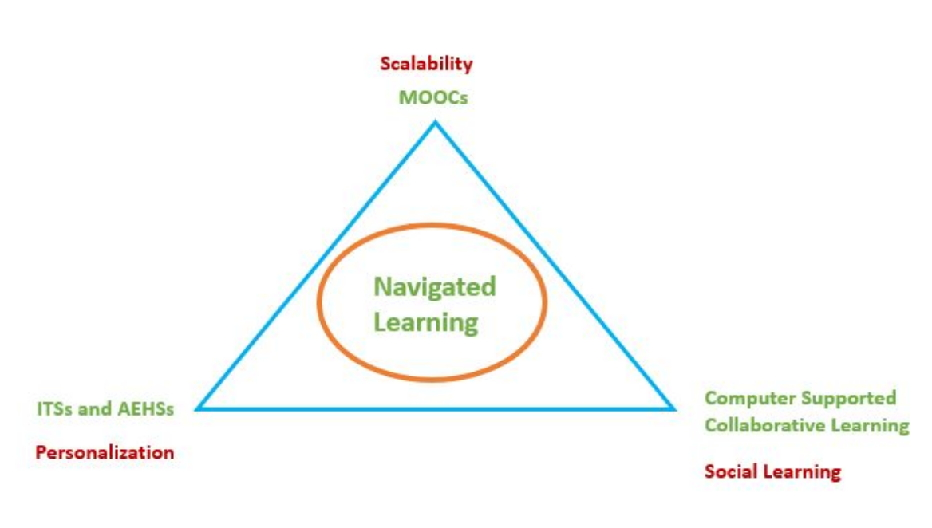
\includegraphics[scale=1.05]{src/Figures/chap2/chap2-fig01.jpg}
\caption{Navigated Learning}\label{chap2-fig01}
\end{figure}

In this article we are characterizing technology-based mediations for navigated learning. For this, initially we discuss the literature about existing solutions MOOCs, ITSs, AEHSs and CSCL that address scalability, personalization and social element of learning. Next, we discuss the concepts such as distributed cognition, ZPD (zone of proximal development), technology based mediated learning and social learning, which are used in technology-based mediations for navigated learning. This is followed by detailed discussion about the pedagogic model for navigated learning and principles of navigated learning. Finally, we present characterization of technology-based navigated learning along with some examples.

\section{MOOC, ITS, AEHS and CSCL}

The MOOC model of learning is the idea of a classroom scaled over a massive student population of all ages. Much of the efforts in this space use the web primarily as an amplifier over existing models of learning, which are based on the classroom. MOOCs have benefitted the environment by lowering the carbon impact, which is calculated by assessing main sources of energy consumption and carbon emissions, including travel, the purchase and use of ICT tools, the consumption of paper and printed materials, residential energy and campus site operations. They have broken economic barriers by lowering the cost of higher education \cite{art2-key29} and socio- cultural barriers by offering education anywhere, anytime, for learners of any age and any culture \cite{art2-key25}. However, MOOCs are criticized for problems, such as high dropout rates, lack of an economically sustainable model, de-skilling the professoriate, cheating and plagiarism \cite{art2-key44}. Other models of online learning, such as ITS and AEHS \cite{art2-key05, art2-key10, art2-key18, art2-key39}, use a one-to-one interface for learning. While reviewing critically ITS and AEHS for collaborative learning support, \cite{art2-key35} mentioned that ITS traditionally focused on curriculum sequencing, intelligent solution analysis and problem-solving support, whereas AEHS focused on navigation and personalized support by using learner models. While the classroom can be described as a pyramid representing a one-to-many relationship between the teacher and the students, called the teacher- student ratio (TSR), ITS and AEHS, represent a one-to-one TSR (Please see Figure~\ref{chap2-fig02}).

\begin{figure}[H]
\centering
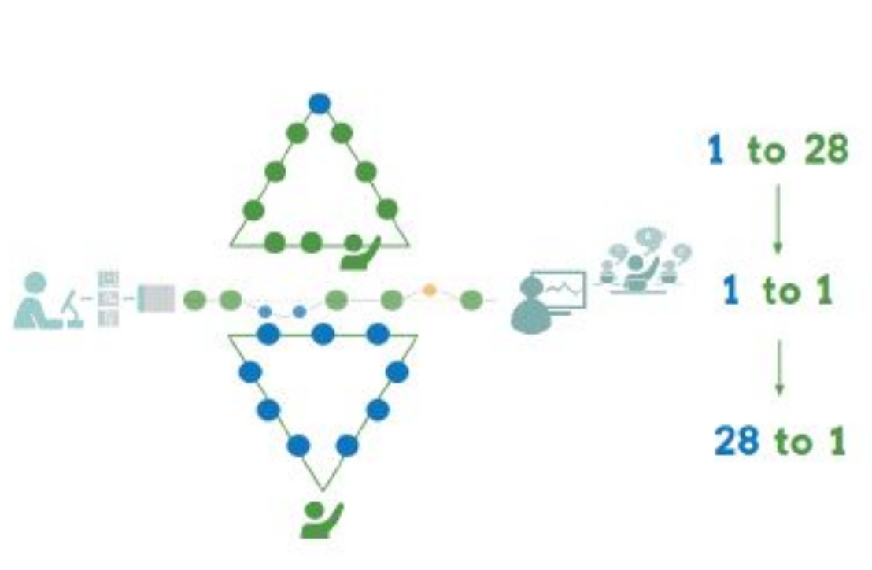
\includegraphics[scale=1.1]{src/Figures/chap2/chap2-fig02.jpg}
\caption{Inversion of the Learning Pyramid}\label{chap2-fig02}
\end{figure}

Further, \cite{art2-key35} argued that the focus of ITS was more on the individual learner, whereas in AEHS, a focus on collaborative learning could be possible. The system design is very important for capturing the peer-interaction (student-student and student-machine) because it highly depends on the design of the system, since we need to get the information from learners implicitly, i.e. without their being conscious of it. The use of AI techniques (such as Bayesian networks \cite{art2-key41}; hidden Markov models \cite{art2-key47}; rule-based and agent- based clustering techniques \cite{art2-key38}; fuzzy and genetic algorithms \cite{art2-key12}) and the semantic social web \cite{art2-key23} to capture and model information for effective monitoring and good support in AEHS would ensure collaborative learning \cite{art2-key35}. The major criticism of ITS and AEHS is that they focus on creating automated tutor agents replacing human teachers by using cognitive science, learning science and artificial intelligence. Hence, the addition of collaborative learning with inclusion of the notions of social web and advanced AI techniques has become a necessity for developing a social learning paradigm.

Collaborative learning refers to students working in collaboration towards obtaining consensus through cooperation, as opposed to working in competition  \cite{art2-key37}. Technology or computer-supported collaborative learning focuses on enhancement of peer interaction and facilitation of distribution of knowledge and expertise  \cite{art2-key33}. In CSCL, the process of collaboration management is informed by one or more computational models of collaborative interaction that provide computer-based representation, helping to understand, explain and predict patterns of group behavior and support the group learning process  \cite{art2-key48}.  \cite{art2-key36} had already foreseen that development of an AI-enabled collaborative learning environment would initiate the use of two key concepts, namely distributed cognition \cite{art2-key20} and Zone of Proximal Development (ZPD) \cite{art2-key51}. \cite{art2-key24} argued that human-computer- interaction should be re-conceptualized as computer-mediated-activity, which leads to further exploration of key notions like technology-based mediated learning (TML), ZPD and distributed cognition.

\section{TML, Distributed Cognition, ZPD and Social Learning}

The term distributed cognition refers to the idea that cognitive processes are distributed across members of social groups, i.e. the processes may be distributed among the coordination between internal structures (i.e. processing and understanding of information) and external structures (i.e. external environment). It is difficult to understand how an individual learns without looking at his/her interactions with other people and artifacts. Cognition happens through interactions between people and artifacts or tools situated in the sociocultural context. In distributed cognition, cognitive processes such as understanding of previous concepts are distributed through time as well, so that earlier events affect later events \cite{art2-key21}. \cite{art2-key45} portrayed organizational cognition as distributed cognition, where people get a rich representation of their knowledge and understanding by self-reflection and communication. The cognitive structures get formed and re-structured through communication and shared understanding. This concerns how the learner learns by using various resources and interacting with those resources, be they humans or artifacts or technology-based resources. \cite{art2-key07} argued that information technology can support distributed cognition by offering ways to communicate, interact, and reflect to form the rich representation of their understanding and restructure the same by reflecting upon and sharing it with others and receiving feedback. The term mediated learning refers to learning with interventions by a mediator (for example, a human expert) and/or through an organized learning activity \cite{art2-key16, art2-key26}. An environment in which the learner’s interactions with learning materials (such as readings, exercises, assignments, peers and/or instructors) are mediated through advanced information technologies is called technology-based mediated learning (TML) \cite{art2-key03}. At the heart of the concept of mediated learning, there is a theory of structural cognitive modifiability (SCM) developed by Feuerstein, which says that a learner’s cognitive structure (i.e. the way s/he learns or her/his intelligence) changes through expert interventions \cite{art2-key27}. Hence, it is also characterized as learning to learn.

Vygotsky \cite{art2-key51} introduced the notion of the social origins of individual psychological functions. He defined the zone of proximal development (ZPD) as the distance between the actual developmental level as determined by independent learning and the level of potential development as determined by the expert’s guidance. In other words, Vygotsky said that while learning, a learner has two performance levels: the level the learner can attain individually and the level the learner can attain with help of an expert. The latter (i.e. the learner’s achievement with the help of an expert) is characterized as ZPD. The theory of ZPD specifies that the development of higher mental processes depends on the presence of the mediating agent that intervenes when a learner is interacting with a learning environment \cite{art2-key26}. The assumption is that as a result of personal interaction in ZPD with the expert, the learner will eventually be able to create a functional system for independent learning.

\cite{art2-key46} argued that Vygotsky’s ZPD is wrongly interpreted as instructional scaffolding, which is actually a contribution of \cite{art2-key55}, and as the notion of ZPD is connected with development through social interaction, which is a long-term continuous process, ZPD should be accurately translated as \textit{zone of next development} (ZND). Suppose a student has learned some concept independently and is struggling to learn some application of that concept. It is more likely that if the student gets some expert’s help, s/he would be able to learn the application of that concept. So, one can say that learning the application of that concept was in the ZPD of that student. The expert’s personality, the nature of the environment, the learner’s cognitive ability to understand the expert’s guidance, and personal traits of the learner - such as being an introvert - have the potential to affect the learning and hence the ZPD of the learner. In technology-based systems, the effects of many of the personality traits of the actors involved and environmental factors could be avoided. By using AI techniques, personality traits could be identified to form groups of learners, and the system could intervene with mediation. ZPD can be the zone where a learner’s potential for new learning is strongest: i.e. it is more effortless and joyful as compared to the zone where the learner finds it very difficult to learn \cite{art2-key14}.

In manual intervention, we cannot ensure the comfort or effortlessness of a student, as these depend on the factors mentioned above. Technology-based systems could help to identify such comfort zones by analyzing the learner’s competencies, preferences, learning styles and other learning profile elements. ZPD can be the range in which a learner can be challenged without causing frustration or loss of motivation \cite{art2-key11}. This is likely to happen when a learner is in a group of peers with whom s/he can be familiar and the interaction is at an equal level and in a friendly manner: such conditions could be found out seamlessly by analyzing the learner’s interaction with the other learners, and even with the teachers and resources with which the learner is learning. The identification of ZPD automatically in TML and mediating is more meaningful than just presenting a learning situation to a learner, where adults or more advanced learners directly or indirectly have a positive influence on the learner \cite{art2-key17}. While studying the dialogic inquiry of sociocultural practice and educational theory, \cite{art2-key54} found the positive role of collaborative learning in the development of ZPD.

Vygotsky \cite{art2-key51} highlighted the role of assistance and collaboration in the development of ZPD, saying that the learner can do more and solve more difficult tasks while collaborating with peers, getting assistance or direction from an expert, or getting some other kind of help, than while working independently. Through collaborative learning, active knowledge construction takes place. Several studies of technology-enabled collaborative learning showed higher levels of interest in learning \cite{art2-key31}; highlighted the engagement of students in deeper levels of thinking \cite{art2-key30, art2-key32}; and reported higher levels of perceived skill development and self-reported learning \cite{art2-key02}. \cite{art2-key52} used conceptual analysis to sharpen the ZPD and concluded that by assigning students tasks which they cannot do alone but can do with peer-assistance, their confidence for independent learning can be developed.

Bandura’s \cite{art2-key06} social learning theory hypotheses that people learn from each other through observation, imitation, and modeling. Social learning is a way to learn other people’s expressions. In social learning, people get signals from other people and use them to infer. This theory is considered a bridge between behaviorist and cognitive learning theories that includes attention, memory and motivation. One cannot learn only with observation and without paying attention. Learning by imitation does not happen without good observation. In social learning theory, it is considered that the learner’s behavior is neither driven by inner forces nor pushed helplessly by influence of the environment but it is result of continuous mutual interaction between behavior and its controlling conditions \cite{art2-key06}. Further, he discussed the effects of concepts such as self-esteem, self- concept and related self-evaluative processes within a social learning framework. So, while designing a technology-based collaborative learning platform for mediation, seamless interaction and learning, the theory of social learning was also found to be grounded and useful. In particular, it provides a basis for user communications as a shifting locus of control for mediation. The interaction of users with each other and with the system provides necessary traction for building balanced interaction and mediation. This is the key to personalization. A mediator is imagined as a hypothetical teacher or a learning resource suggested by the system or a tutor or peers. Mediated learning is about developing conscious awareness and volition among learners about learning. It is more towards encouraging learners for learning through personalized interventions, i.e. by considering each learner’s comfort zone. When we consider a social learning platform from the network point of view, the emergence of a network through interaction is the prime driver for further interaction among people. Thus, technology-based mediations in navigated learning has the potential to invert the learning pyramid by interfacing the learner with several experts (i.e. the many-to-one TSR model) as part of a single learning experience shown in Figure~\ref{chap2-fig02}.

\section{Navigated Learning}

The primary idea behind Navigated Learning that addresses all three concerns of scale, individualization and social elements of learning, is called \textit{semantic embedding} in a \textit{progression space}. We will describe both these terms in this section.

\subsection{Pedagogic Model for Navigated Learning}

The pedagogic model for navigated learning is based on embedding learning resources, learner competencies and any other artifact relevant to the learning process, into a logical progression space called the learning map.

A \textit{progression space} represents an area– specifically, a metric space, through which, several participants progress through time. The design of such spaces is meant to facilitate progressions for all participants, in as close to an optimal fashion as possible. Examples of progression spaces from other spheres of life include: airports, metro train stations, bus stations, fast-food outlets, etc. Such spaces are characterized by a floating population of individuals (also called \textit{participants}, or, in our case, \textit{learners}), each pursuing disparate goals, but of a largely similar nature. There need not be one common, overarching goal being pursued by the entire population. For instance, not all people in a bus station may be going to the same destination, but most of the participants in a bus station are there because they want to go somewhere or are arriving from somewhere.

Formally, a progression space is defined as follows:
\begin{figure}[H]
\centering
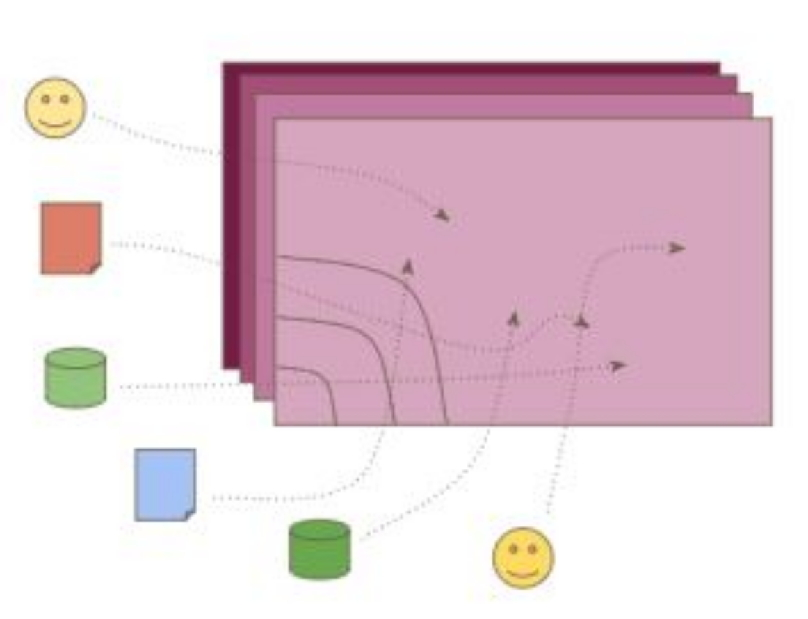
\includegraphics[scale=1.2]{src/Figures/chap2/chap2-fig03.jpg}
\caption{Progression Space for a Subject}\label{chap2-fig03}
\end{figure}
\vskip -.5cm
\begin{equation}
S=(C, d, \preceq)\label{eqn-1}
\end{equation}

Here $C$ is a set of points that make up the space, $d : C \times C → \Re$ is a “distance” function between any pair of points in the space. A distance function has the following characteristics:

\noindent
\begin{tabular}{@{}r@{~~}c@{}}
\textit{Reflexivity} &  $\forall x \in C, d(x, x) = 0$\\[3pt]
\textit{Symmetry} &  $\forall x, y \in C, d(x, y) = d(y, x)$\\[3pt]
\textit{Triangle inequality} & $\forall x, y, z \in C, d(x, z)\leq d(x, y) + d(y, z)$
\end{tabular}

The term $\preceq \subseteq C \times C$ in Eqn~\ref{eqn-1} represents a “progression” relationship between pairs of points. A relationship of the form $c_1 \preceq c_2$ represents that a learner at point $c_2$  has progressed at least as much as learner $c_1$. 

Actions and states of participants in a progression space are not necessarily independent of one another. The presence of some participant in some part of the space may (positively or negatively) affect the experience of other participants nearby.

Navigated learning characterizes learning as an aided navigation through a progression space comprising of several learning activities and other learners. The journey of a learner is curated by a navigator software, based on the learner’s goals. The navigator not only aims to personalize the learning pathway for the learner’s needs, it also tries to take advantage of the presence of other participants in the system.

The unit of activity in this space, is called a \textit{learning activity}. A learning activity includes but is not limited to, consuming of resources like videos or lecture notes. A given learning activity may also involve several learners participating in a synchronous fashion, like in a group discussion or a debate. A learning activity also need not be a purely online activity. It can even be an offline activity, like attending a lecture in a conventional classroom. The only requirement for a learning activity is that it should \textit{generate activity data} that helps the navigator locate and navigate the learner in the space.

Offline learning activities that are part of a navigated learning scheme, are designed such that they contain mechanisms to generate relevant activity data, and push them to the backend that is managing the navigated learning. These mechanisms include smartphone apps that learners install, which records and transmits their activity details, or even low tech mechanisms like a teacher collecting data from students after every learning activity, and uploading them in bulk.

Figure~\ref{chap2-fig03} depicts a semantic progression space for any given subject. Any subject matter of study is divided into one or more \textit{facets} of study. Each of facet is represented by a 2-dimensional progression space.

A progression space for subject $S$ and facet $f$ , is represented as a 2-dimensional \textit{competency map} that is formally defined as follows:
\begin{equation}
CM(S_f)=(C, P, Q ,\gamma , d,\preceq)\label{eqn-2}
\end{equation}

Here the term $C$, which is the set of points forming the progression space, represents a set of \textit{competencies} that are the basic unit of learning. The terms $P$ and $Q$ represent the horizontal and vertical axes of the progression space respectively. The horizontal axis represents a set of topics (also called “domains”) that are addressed as part of this facet. The vertical axis represents the depth or “level” at which a particular topic is studied. Higher values of $Q$ represents more depth, requiring a higher level of skill and comprehension. The terms $d$ and $\preceq$ represent the distance and progression maps, as described in Eqn~\ref{eqn-1}. The $P$ and $Q$ coordinates are organized such that progression is always from left to right, and bottom to top. Hence, for any pair of competencies $c_1 , c_2 \in C, c_1 \preceq c_2 \Rightarrow p(c_1 )\leq p(c_2 )$ and $q(c_1 ) \leq q(c_2 )$, and for at least one of the dimensions $x \in \{p, q\}, x(c_1 ) < x(c_2 )$. In the figure, this property is schematically depicted as concentric arcs, emanating from the bottom-left to the top-right.

The term $\gamma : C \rightarrow P \times Q$ represents an embedding function for competencies that assigns a $(p, q)$ coordinate for each competency. The actual form of the embedding function itself is not specified by the navigated learning framework. The only constraint for the embedding function is that it should preserve the progression property from bottom-left to top-right.

A \textit{learning map} for a given progression space comprises of a set of \textit{learning activities} that are embedded into the space. Formally:
\begin{equation}
LM(S_f ) = (S_f , A, \delta, L)\label{eqn-3}
\end{equation}

Here $A$ is a set of learning activities, and $\delta : A \rightarrow S_f $ embeds each learning activity by mapping it onto a competency in $S_f$ . A learning activity is an abstract container that encapsulates several kinds of learning engagements. For a given learning activity $a \in A$, the term \textit{typeof (a)} is used to ascertain what kind of learning activity it is.

As earlier, the navigated learning framework itself does not prescribe any specific technique for embedding learning activities into a competency space. The only semantic requirement is that a learning activity $a$ mapped to a competency $c$ should be useful for a learner in acquiring the competency $c$. In early implementations of navigated learning in K-12 settings, learning activities were manually embedded onto the space by experts. Later on, using this as a training dataset, machine learning algorithms were built to embed learning activities.

Each embedding of the form $\delta (a) = c$, represented by the tuple $(a, c)$ is associated with it, several kinds of meta-data. Some of these are as follows
\begin{description}
\item[Relevance:] The relevance function \textit{relevance:} $A \times C \rightarrow [0, 1]$ measures the fit between the learning activity and the competency to which it is mapped to.
\item[Engagement:] This is a score of the form  \textit{engagement}: $A \times C \rightarrow [0, 1]$ that rates the learning activity with respect to other learning activities mapped to the same competency $c$ for relative popularity of it being used in any learning pathway.
\item[Efficacy:] This is a score of the form \textit{efficacy:} $A \times C \rightarrow [0, 1]$ that tries to estimate the probability that a given learner would obtain competency $c$, by performing learning activity $a$.
\end{description}

A set of data-driven interpretations for these metrics, and corresponding algorithms for computing these metrics are detailed in Ram and Srinivasa \cite{art2-key40}.

The term $L$ in Eqn~\ref{eqn-3} represents a set of \textit{learning pathways} that are part of the learning map. A learning pathway $l \in L$ is a sequence of competencies $l \in C^\ast$ that represents a coherent and progressive learning sequence. A learning pathway is a feature of the learning map, rather than that of a learner. That is, a learning pathway need not have a specific stated goal, and is not customized for a given learner. It only represents a coherent sequence of competencies. The formal notion of coherency of a learning pathway is called the “Narrative Arc”.

\subsection{Principles of Navigated Learning}

With the necessary definitions for semantic embeddings in a progression space, we now describe the principles of navigated learning. Navigated learning can be summarized by the following steps: \textit{Locate, Curate, Mediate.}

Navigated learning is manged by a “Learning Navigator” with which every learner interacts. The Learning Navigator (or just, navigator), continuously interacts with the learning map and the learner to perform the following:
\begin{description}
\item[Locate:]  Based on data about their activities and outcomes from formal assessments, the “Locate” module of the navigator embeds learners in the space, and continuously updates their location. Unlike a geographical space, a learner may have acquired several competencies in the competency space. Thus, their location is not identified by a point, but by a data structure called a \textit{Skyline}, that is detailed in a later section.
\item[Curate:] Once a learner’s location is known, based on their stated goals or recently acquired competencies, a set of further candidate competencies are identified. Curating is based on competency modeling principles, that identifies complementary, supplementary and conflicting competencies.
\item[Mediate:] This is the logic by which the navigator navigates the learner by making suggestions. Mediation is based on computing an underlying “Narrative Arc” that computes a semantically coherent and meaningful learning sequence individualized for each learner. Mediation also involves suggesting connections with other learners as well as group learning activities.
\end{description}

In addition to the above, when learners interact with a learning map, they can explore the learning space as if it were a 2D shared physical space. They can browse through the space, and encounter learning activities, resources, as well as other learners at different points in the space. They can follow pre-computed learning pathways to go through a coherent sequence of activities.

Every resource would be classified for instructional practice (classification based on its possible use for introduction or learning or practice or assessment of a concept), and its rigor (the fine line between challenging and frustrating a student, i.e. students are challenged to think, perform and grow to a level different from their earlier level) would be identified by using machine learning techniques. Also, for all resources a coherence (similarity) score between any two resources would be computed, and this could be used for defining the proximity between the two resources and even a learning path (a sequence of resources given by a teacher) that uses those resources. For every resource, relevance and engagement scores would be computed with respect to any competency based on how many times a resource is used/reused by a curator for a competency (how relevant the resource is found) and the number of likes and ratings the resource has received from various learners for a competency (how engaging the resource is found). By combining both the relevance and the engagement score of a resource, the efficacy score of that resource with respect to a competency would be computed by using some algorithm.

Learners may be part of a formal classroom or a group or may learn independently for his/her informal learning. Learners would interact with a resource or collection of resources in order to obtain a competency. A social interaction forum would be included in the system, where, while interacting with a resource or a collection of resources, learners can interact with each other, collaborate, discuss, ask and answer questions, and rate and like the questions and answers. Learners can express themselves with personalized learning stories, do peer-grading and evaluation, and tag peers. Every interaction of a learner with the system - i.e. with peers, with resources and with a hypothetical teacher will be a data point for capturing evidence for a learner’s competency. The full range of learner activities would be aggregated, e.g. assessments activities, social interactions, sharing and expression, etc. (posting a question and answering a question on a discussion forum are both learning activities). The data from these activities would be analyzed using the appropriate analysis tools. All data aggregated from learning  activities need to be processed prior to use, e.g. text analysis, sentiment analytics, assessment feedback/scores analysis. We would store the data so that we can support visualization, personalize pathways, and manage goals and interactions among learners.

\newpage

A learner profile would be visualized by Activity, Time, Learning Situation, User-groups, Performance for a learner. ATCUP are defined as: Activities by type (Study, Course Building, Community, Portfolios), time drill- downs (All-time, Year, Month, Week, Day), Learning situation (subject, course, professional skill), User-Groups (User, Class, Groups, Grade within and across schools, organizations, etc.), Performance (Effort, Credentials and badges, Proficiency, Authority, Citizenship, Tags). Basic information such as role (teacher, student), grade, curriculum standard, etc. and context as a weighted average of the competency that the user has engaged in recently, will be part of the profile, but captured under tags for user vectors. This would average the different topics that the learner has spent time studying, weighted by the amount of time spent and recency. Context would also include the learner’s preference, which will be computed based on their relative time spent on subjects or topics and resource types. A learner’s learning style would be identified automatically by using AI techniques.

A learner’s progress would be based on earned competencies in the system, and on the inferred competencies and the asserted competencies of the learner. Competencies would be either completed (by earned, inferred or asserted), in-progress or not-started and would be represented as a part of learner proficiency in the report. Learner proficiency would be represented as a competency skyline in a learning map (please see Figure~\ref{chap2-fig04}). A skyline algebra enables reasoning about competencies acquired by a population of learners. The user vector includes the authority, citizenship and reputation of a user and would be computed based on the given definitions. A good authority will be the one who contributes learning content and creates courses and learning activities. The authority score will also be boosted by how well they are recognized by other learners. A good authority will be one who is recognized by good citizens. A good citizen will be one who recognizes good authorities by responding to the content/activities created by them. The reputation of a user will be based on the number of likes, ratings and followings another user has given for her/his contributions. A learner will be able to set and manage learning goals. The system will be able to show a learner’s performance against her/his learning goals.

The analyzed data from a variety of learner activities will be used to compute the user vector. These vectors will be used in path-planning algorithms. Every user will create and evolve the profile based on their activities. Users start with basic information about their name and email-id. As they study, create or curate courses, and interact with other users, their profile evolves toward the system gaining a full understanding of the user. Besides consuming learning, learners will contribute to supporting other users with activities such as sharing, peer-grading, reviewing contributions to moderate for quality, etc. The idea of being a contributor to the learning system would give traction for increased communication. All this information captured would be used for learning
mediations.

\section{Characterization of Technology-Based Mediation for Navigated Learning}

The suggest sub-system (described in \cite{art2-key28}) of the described navigated learning paradigm defines how technology-based mediation would be carried out. While curating the content in the learning navigator, a teacher can specify a learning path. The system also suggests a learning path based on a learner profile built by its deep-end (described in \cite{art2-key28}) combined with the information obtained through Event-Condition-Action (ECA) rules. The suggest system intervenes in several such workflows on a continuous basis, based on semantics extracted from systemic activities. Suggest algorithms are triggered by ECA rules embedded in different parts of the system. The suggest trigger may intervene not just in the student’s learning pathway, but also in the workflows of other pertinent stakeholders like the teacher, course content creator, etc.

\vskip -.3cm

\begin{figure}[H]
\centering
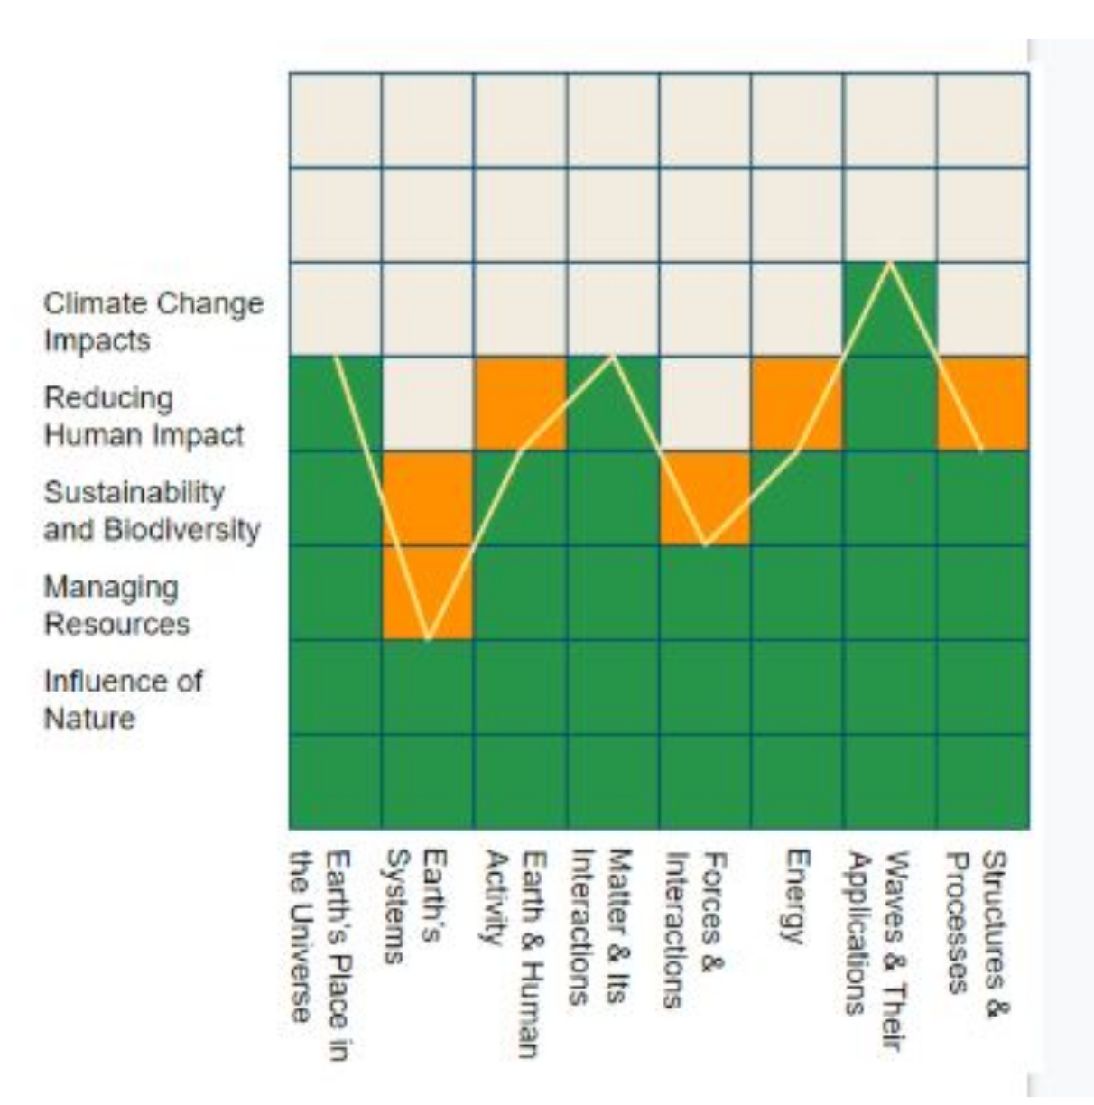
\includegraphics{src/Figures/chap2/chap2-fig04.jpg}
\caption{Example of a facet in a Learning Map as a 2D Space}\label{chap2-fig04}
\end{figure}

\vskip -.6cm

The basic prerequisites for achieving the vision discussed earlier include the capability to locate the learner, curate potential learning activities, and make appropriate suggestions based on their context. The suggest sub-system leverages key elements from learning science, cognitive science and data science to design the most precise learning pathway for every learner. This requires multivariate optimization across different learning pathways based on learning, cognitive and data sciences. We categorize learning mediations into two major types: \textit{fully automated mediation and semi-automated peer-driven mediation.} These two types of mediations can be characterized in detail based on elements such as relevance, engagement, efficacy, authority, citizenship, learner context (i.e. the context in which the learner is), learner characteristics and learner profile.

\subsection{Fully Automated Mediations}

We consider the learning navigator as a hypothetical teacher who is observing the learner continuously, and also as a mediator that suggests learning resources automatically. This approach of mediations we name fully automated mediation. After determining the location of that learner for the domain on the learning map, the system would identify the ZPD/ ZND of the learner, which would be used for mediation. A few heuristics of these characterizations are given in Figure~\ref{chap2-fig05}, Figure~\ref{chap2-fig06}, Figure~\ref{chap2-fig07}. In these fully automated mediations, the system acts as mediator, a hypothetical teacher who understands the learner. By using the available data about a learner and the available resources, her/his ZPD (set of competencies) would be identified, and the same would be used for mediation. Identification of ZPD automatically by using one or more data points is crucial for mediation. The very basic way to identify ZPD is through the immediate progressions (i.e. connected competencies) of a mastered (80\% performance) competency.
\begin{figure}[H]
\centering
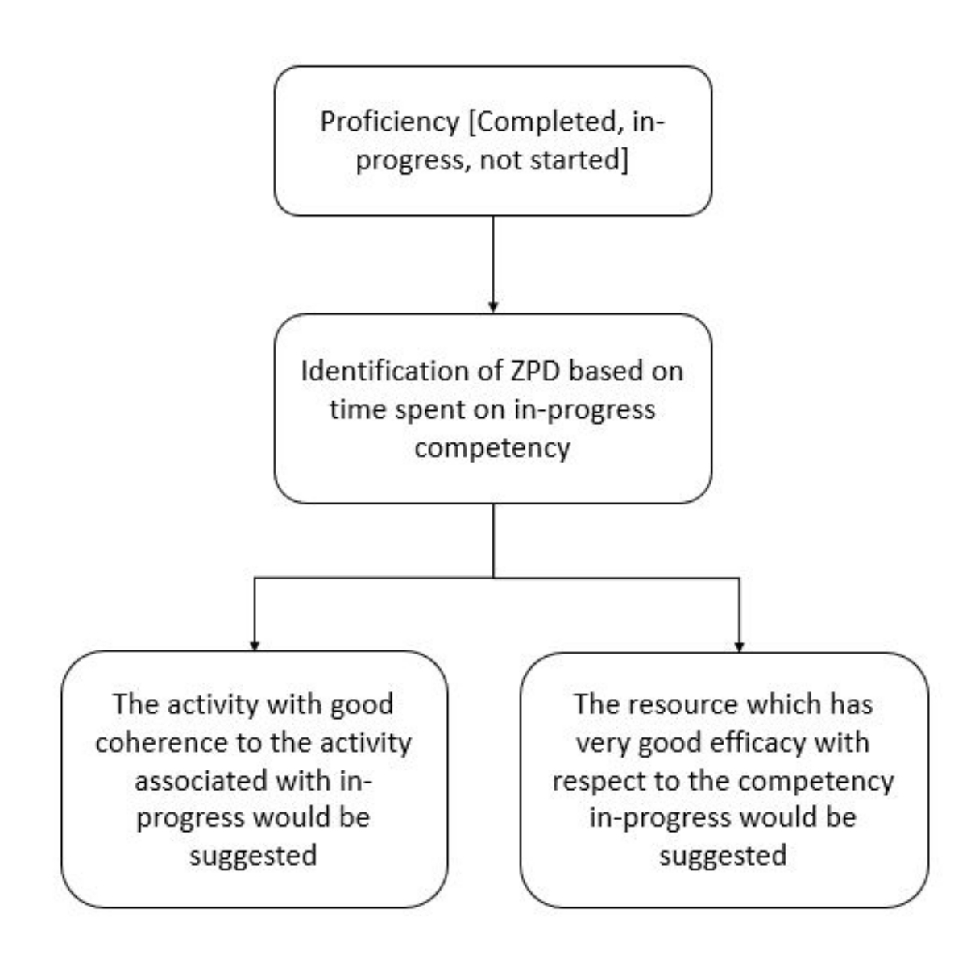
\includegraphics[scale=.75]{src/Figures/chap2/chap2-fig05.jpg}
\caption{Fully Automatic Mediation Heuristic (a)}\label{chap2-fig05}
\end{figure}

\begin{figure}[H]
\centering
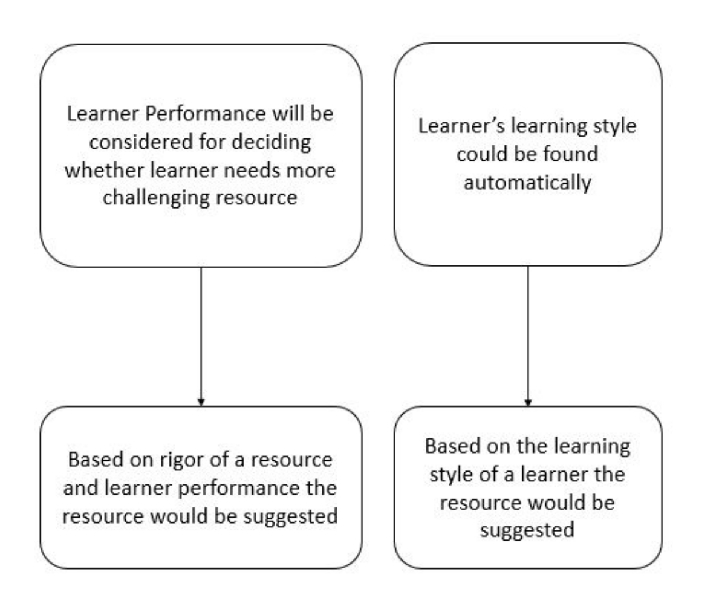
\includegraphics{src/Figures/chap2/chap2-fig06.jpg}
\caption{Fully Automatic Mediation Heuristic (b)}\label{chap2-fig06}
\end{figure}

\begin{figure}[H]
\centering
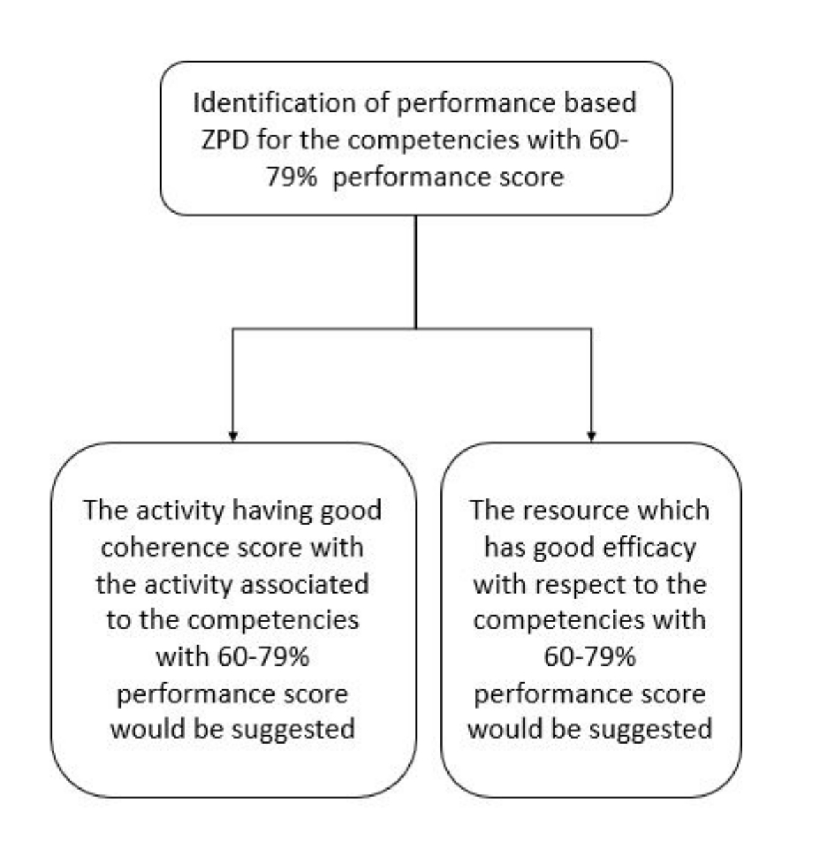
\includegraphics[scale=.85]{src/Figures/chap2/chap2-fig07.jpg}
\caption{Fully Automatic Mediation Heuristic (c)}\label{chap2-fig07}
\end{figure}

Competencies for which the performance of a learner is within the 60-79\% range would be identified as the learner’s ZPD. The set of competencies associated with the resources that are most coherent with the resources associated with a mastered competency would be considered as a possible ZND for a learner. We can also identify the ZND of a learner based on time spent on the in-progress competencies in a learning map. Learner scores like authority, citizenship, and reputation, together with user preferences, would be considered for identifying a ZPD.

\subsection{Semi-automatic Peer-driven\hfill\break Mediations}

In these mediations, the suggestions and the point of suggest would be identified automatically by the system making use of the information gathered through learner interactions to the system. These suggestions would be put forward to the teachers, peers and the freedom to consider the suggestions is left to them. That is why we call it semi-automatic and peer-driven mediations.

By considering the inputs from distributed cognition, we also consider the other users - i.e. the peers and even the teacher - as another set of mediators. The system will suggest to these mediators the learning resource and the point of mediation, i.e. the point where an intervention could be made. These mediators can use their own judgement to accept the suggestion or consider something else. These mediators would be decided automatically by the system based on their interaction among each other, and hence this kind of mediation by these mediators is named semi- automated peer-driven mediation. After identification of ZPD of a user automatically, the system would suggest a peer or a group of peers to a user for further interaction. A few heuristics for this characterization are given in Figure~\ref{chap2-fig08}, Figure~\ref{chap2-fig09}, Figure~\ref{chap2-fig10}.
\begin{figure}[H]
\centering
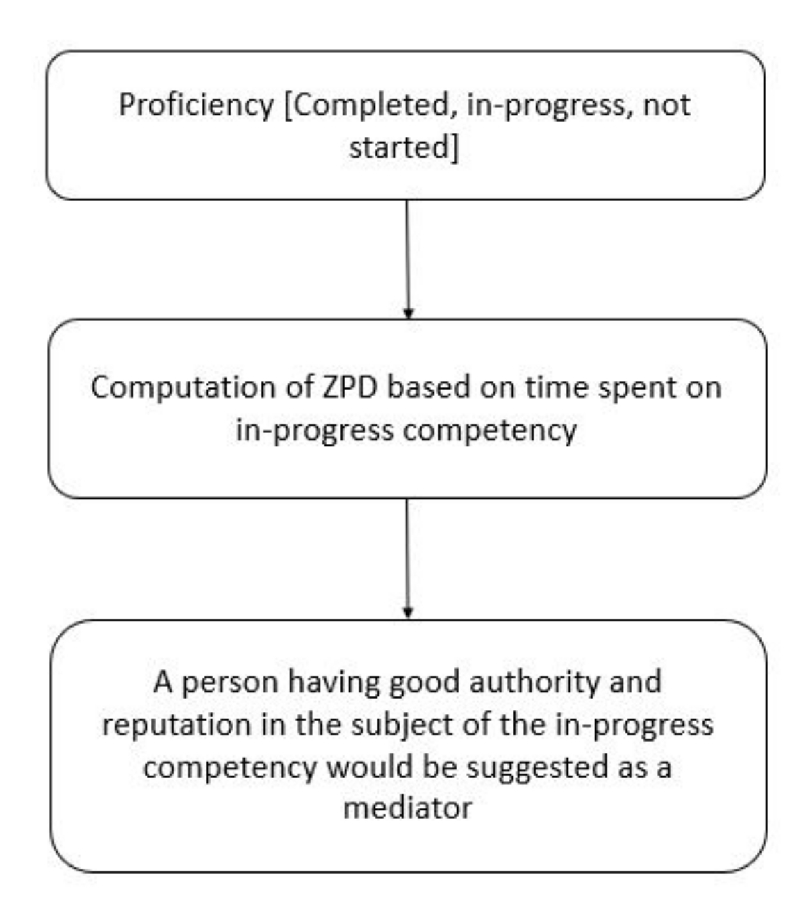
\includegraphics[scale=.85]{src/Figures/chap2/chap2-fig08.jpg}
\caption{Semi-automatic Peer-driven Mediation Heuristic (a)}\label{chap2-fig08}
\end{figure}

\vskip -.5cm

\begin{figure}[H]
\centering
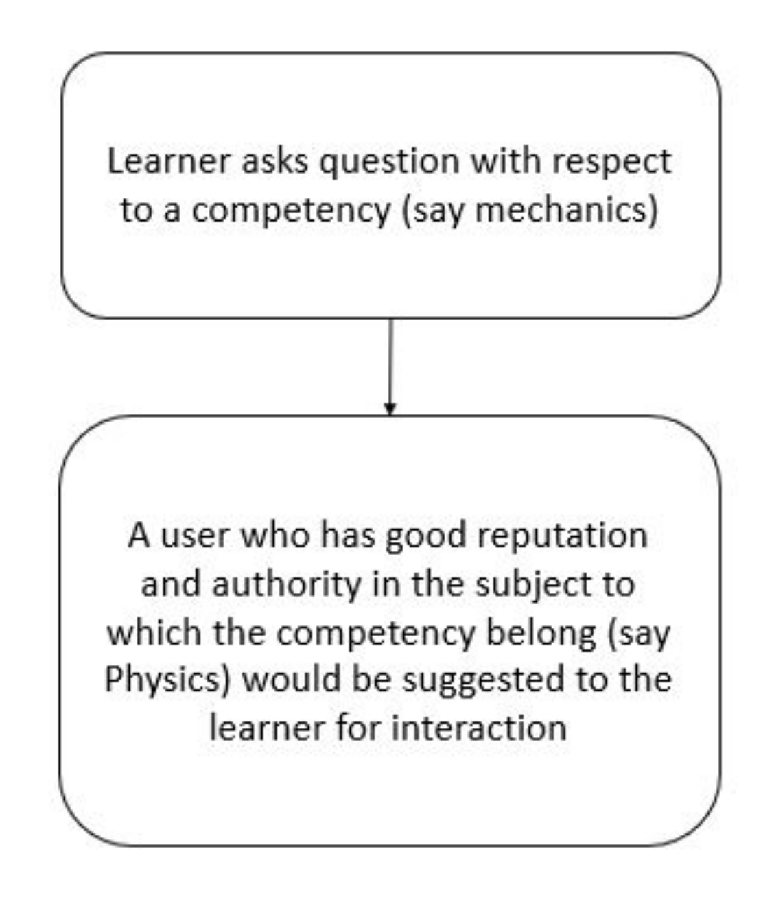
\includegraphics[scale=.77]{src/Figures/chap2/chap2-fig09.jpg}
\caption{Semi-automatic Peer-driven Mediation Heuristic (b)}\label{chap2-fig09}
\end{figure}

\begin{figure}[H]
\centering
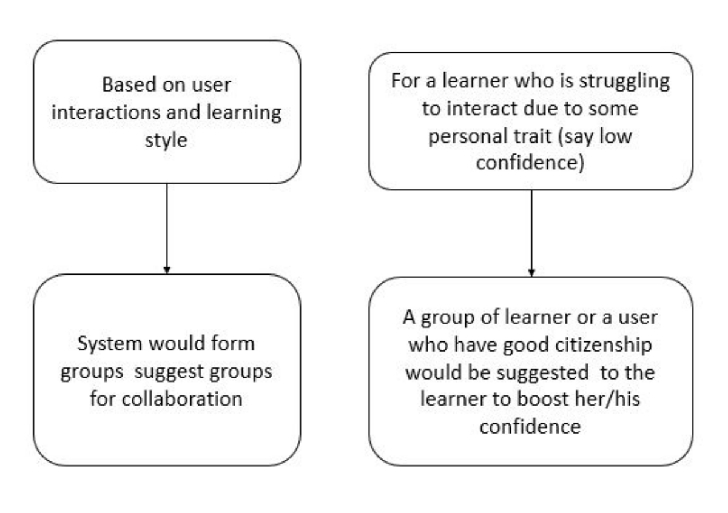
\includegraphics[scale=1.35]{src/Figures/chap2/chap2-fig10.jpg}
\caption{Semi-automatic Peer-driven Mediation Heuristic (c)}\label{chap2-fig10}
\end{figure}

The essence of cooperative learning is students learning in groups, which increases motivation and improves interrelationships and as positive effects on achievements and higher-order thinking \cite{art2-key13}. Considering group dynamics, the system can identify groups in which good students dominate and may thus affect the performance of the whole group in a positive manner, the system can then suggest that a lower-performance learner in a subject should be part of a group with high-performing students in that subject who have good citizenship and reputation.

Even after the mediation with basic heuristics, the system would observe the learner to see the effect of the mediation. If the mediation is effective, then the system would remember that heuristic as a validated strategy, and if the mediation is found to be ineffective, then it would remember this and adjust the mediation with another heuristic. There could be pre-defined heuristics, or the system could learn the heuristics for mediation from user interactions. Thus, mediations by the system would be controlled by the user interaction with the system, i.e. learning resources and peers. Usually, adaptive systems are pre-designed for adaptation of the content and offering the content in a personalized manner to the user. So, an adaptive system’s control is always only with  the system and hence its design. In the proposed system, user interaction with the system is the prime driver for emergence of the network, and hence these medications are adjusted as per user interaction. So, mediations would not be controlled single handedly by a user or even by a system. In a technology- based mediated social learning platform, the mediation will be a balanced control between the system (the hypothetical teacher) and the users. Hence, the proposed system for social learning could invert the learning pyramid and can be considered a many-to-one TSR model.

\vfill\eject

\section{Discussion}

For MOOCs, the notion of connectivist MOOCs (cMOOCs) emphasizing collaborative learning and knowledge construction by a learner community exists at conceptual level \cite{art2-key56}. In the MOOCs such as Coursera and Edx collaborative learning is implemented (in a few courses) by using discussion forums and peer assessments. Still there are no evidences available to show how these have addressed challenges such as high dropout rates, lack of an economically sustainable model, de-skilling the professoriate, cheating and plagiarism. The proposed model encourages voluntary participation as part of a social learning community that constructs knowledge. The voluntary participation and it being associated more with self-learning discards possibilities of cheating, plagiarism and dropouts. In the proposed model, there is no single professor teaching one full course to a set of learners, and the system uses open educational resources (OER) with emphasis on the group of users contributing towards learning.

Conversational ITSs such as AUTOTUTOR \cite{art2-key19} and ATLAS \cite{art2-key50} have dialogue between the machine tutor and the learner. These use production rule-based question answering systems, and learner information is gathered from the learner’s expressions, synthesized speech, intonation and gestures. In these ITSs, the mediation is fully automated by the machine tutor, but based on predefined production rules. There is no element of collaborative learning and knowledge construction in these ITSs. The proposed model includes seamless user interactions and the mediation is fully automated based on the data gathered by machine-learning techniques, data science and semi-automated peer-driven for which each learner’s ZPD is identified and used for mediation. It does not remain just a technology-based personalized platform, but a social machine into which notions like distributed cognition and social learning are being incorporated. In AEHS such as ELM-ART \cite{art2-key53}, the mediation is based on logical models pre-defined by the system designer, and no element of collaboration or peer-interaction is included. The control of mediation is only with the system and not with the user using the system. In the proposed model and system, mediation is a balanced control between the user and the system and is not controlled by either the user alone or the system alone. In the CSCL systems \cite{art2-key48}, the mediation for supporting collaborative learning is mainly based on the understanding of the group activity, the group behavior, and also considers an individual’s ZPD. CSCL systems do not have fully automated mediation, whereas our proposed model includes both, i.e. fully automated and semi-automated peer-driven mediation.

\bigskip
\bigskip
\medskip

\section{Summary and Conclusion}

This article has described a pedagogic model based on technology-based mediation for navigated learning and characterized the technology-based mediation. These mediations could be used in the learning navigator, where the web acts as a platform to nurture a learning community by continuously mediating between knowledge need and expertise through a mechanism called suggest sub-system. We foresee the learning navigator as a TML platform that can identify a learner’s ZPD and provide guidance to the learner on how to learn through personalized interventions. The learning navigator considers, every situation as a learning situation and models it into a scientific learning experience. The navigated learning has the capability to invert the learning pyramid from a one-to-many TSR model to a many-to-one TSR model. Since it is a technology-based platform, irrespective of the mode of using technology, it can make a learner more curious and inspire her or him to fall in love with learning. We also compared the proposed approach with existing models of technology-based education and discussed how the proposed system can counter the challenges faced by MOOCs, ITSs and AEHSs. Navigated learning has the potential to leverage the power of technology to amplify the learning ability of a learner, providing an experience of being part of a learning community of teachers, experts and peers.\raisebox{-.1cm}{
\includegraphics[scale=.9]{src/Figures/circledC.eps}}

\begin{thebibliography}{99}
\bibitem{art2-key01} 2017. Beyond Basics: National Findings. (2017), 56–62.
\bibitem{art2-key02} Maryam Alavi. 1994. Computer-mediated collaborative learning: An empirical evaluation. \textit{MIS quarterly} (1994), 159–174.
\bibitem{art2-key03} Maryam Alavi and Dorothy E Leidner. 2001. Research commentary: Technology-mediated learning, A call for greater depth and breadth of research. \textit{Information systems research} 12, 1 (2001), 1–10.
\bibitem{art2-key04} Vincent Aleven, Bruce M Mclaren, Jonathan Sewall, and Kenneth R Koedinger. 2009. A new paradigm for intelligent tutoring systems: Example-tracing tutors. \textit{International Journal of Artificial Intelligence in Education} 19, 2 (2009), 105–154.
\bibitem{art2-key05} John R Anderson, C Franklin Boyle, and Brian J Reiser. 1985. Intelligent tutoring systems. \textit{Science} 228, 4698 (1985), 456–462.
\bibitem{art2-key06} Albert Bandura and Richard H Walters. 1977. \textit{Social learning theory.} Vol. 1. Prentice-hall Englewood Cliffs, NJ.
\bibitem{art2-key07} Richard J Boland Jr, Ramkrishnan V Tenkasi, and Dov Te’eni. 1994. Designing information technology to support distributed cognition. \textit{Organization science} 5, 3 (1994), 456–475.
\bibitem{art2-key08} Lori Breslow, David E Pritchard, Jennifer DeBoer, Glenda S Stump, Andrew D Ho, and Daniel T Seaton. 2013. Studying learning in the worldwide classroom research into edX’s first MOOC. \textit{Research \& Practice in Assessment} 8 (2013), 13–25.
\bibitem{art2-key09} Peter Brusilovsky. 2001. Adaptive educational hypermedia. In \textit{International PEG Conference,} Vol. 10. 8–12.
\bibitem{art2-key10} Peter Brusilovsky. 2003. Developing adaptive educational hypermedia systems: From design models to \textit{authoring tools. In Authoring tools for advanced technology Learning Environments.} Springer, 377–409.
\bibitem{art2-key11} Seth Chaiklin. 2003. The zone of proximal development in Vygotsky's analysis of learning and instruction. \textit{Vygotsky's educational theory in cultural context} 1 (2003), 39–64.
\bibitem{art2-key12} Raquel M Crespo, Abelardo Pardo, Juan Pedro Somolinos Pérez, and Carlos Delgado Kloos. 2005. An algorithm for peer review matching using student profiles based on fuzzy classification and genetic algorithms. In \textit{International Conference on Industrial, Engineering and Other Applications of Applied Intelligent Systems.} Springer, 685–694.
\bibitem{art2-key13} Zoltán Dörnyei. 1997. Psychological processes in cooperative language learning: Group dynamics and motivation. \textit{The Modern Language Journal} 81, 4 (1997), 482–493.
\bibitem{art2-key14} Richard Fabes, Carol Lynn Martin, et al. 2001. \textit{Exploring development through childhood.} Allyn \& Bacon.
\bibitem{art2-key15} Richard M Felder, Linda K Silverman, et al. 1988. Learning and teaching styles in engineering education. \textit{Engineering education} 78, 7 (1988), 674–681.
\bibitem{art2-key16} Reuven Feuerstein, Mildred B Hoffman, Yaacov Rand, Mogens R Jensen, David Tzuriel, and David B Hoffmann. 1985. Learning to learn: Mediated learning experiences and instrumental enrichment. \textit{Special Services in the Schools} 3, 1-2 (1985), 49–82.
\bibitem{art2-key17} Julia Gillen. 2000. Versions of Vygotsky. \textit{British Journal of Educational Studies} 48, 2 (2000), 183–198.
\bibitem{art2-key18} Arthur C Graesser, Mark W Conley, and Andrew Olney. 2012. Intelligent tutoring systems. (2012).
\bibitem{art2-key19} Arthur C Graesser, Katja Wiemer-Hastings, Peter Wiemer-Hastings, Roger Kreuz, Tutoring Research Group, et al. 1999. AutoTutor: A simulation of a human tutor. \textit{Cognitive Systems Research} 1, 1 (1999), 35–51.
\bibitem{art2-key20} James Hollan, Edwin Hutchins, and David Kirsh. 2000. Distributed cognition: toward a new foundation for human-computer interaction research. \textit{ACM Transactions on Computer-Human Interaction (TOCHI)} 7, 2 (2000), 174–196.
\bibitem{art2-key21} Edwin Hutchins. 2000. Distributed cognition. \textit{International Encyclopedia of the Social and Behavioral Sciences. Elsevier Science} 138 (2000).
\bibitem{art2-key22} Patrick Jermann and Pierre Dillenbourg. 2008. Group mirrors to support interaction regulation in collaborative problem solving. \textit{Computers \& Education} 51, 1 (2008), 279–296.
\bibitem{art2-key23} Jelena Jovanović, Dragan Gašević, Carlo Torniai, Scott Bateman, and Marek Hatala. 2009. The Social Semantic Web in Intelligent Learning Environments: state of the art and future challenges. \textit{Interactive Learning Environments} 17, 4 (2009), 273–309.
\bibitem{art2-key24} Victor Kaptelinin. 1996. Computer-mediated activity: Functional organs in social and developmental contexts. \textit{Context and consciousness: Activity theory and human-computer interaction} (1996), 45–68.
\bibitem{art2-key25} Hanan Khalil and Martin Ebner. 2014. MOOCs completion rates and possible methods to improve retention-A literature review. In \textit{EdMedia: World Conference on Educational Media and Technology.} Association for the Advancement of Computing in Education (AACE), 1305–1313.
\bibitem{art2-key26} Alex Kozulin. 2003. Psychological tools and mediated learning. \textit{Vygotsky's educational theory in cultural context} (2003), 15–38.
\bibitem{art2-key27} Alex Kozulin, Jo Lebeer, Antonia Madella-Noja, Fernando Gonzalez, Ingrid Jeffrey, Naama Rosenthal, and Mennyi Koslowsky. 2010. Cog-nitive modifiability of children with developmental disabilities: A multicentre study using Feuerstein’s Instrumental Enrichment Basic program. \textit{Research in Developmental Disabilities} 31, 2 (2010), 551–559.
\bibitem{art2-key28} Aparna Lalingkar, Srinath Srinivasa, and Prasad Ram. 2018. Deriving Semantics of Learning Mediation. In \textit{2018 IEEE 18th International Conference on Advanced Learning Technologies (ICALT).} IEEE, 54–55.
\bibitem{art2-key29} Andy Lane, Sally Caird, and Martin Weller. 2014. The potential social, economic and environmental benefits of MOOCs: operational and historical comparisons with a massive closed online course. \textit{Open Praxis} 6, 2 (2014), 115–123.
\bibitem{art2-key30} Erno Lehtinen. 2003. Computer-supported collaborative learning: An approach to powerful learning environments. \textit{Powerful learning environments: Unravelling basic components and dimensions} 35 (2003), 54.
\bibitem{art2-key31} Dorothy E Leidner and Mark Fuller. 1997. Improving student learning of conceptual information: GSS supported collaborative learning vs. individual constructive learning. \textit{Decision Support Systems} 20, 2 (1997), 149–163.
\bibitem{art2-key32} Kai H Lim, Lawrence M Ward, and Izak Benbasat. 1997. An empirical study of computer system learning: Comparison of co-discovery and self-discovery methods. \textit{Information Systems Research} 8, 3 (1997), 254–272.
\bibitem{art2-key33} Lasse Lipponen. 2002. Exploring foundations for computer-supported collaborative learning. In \textit{Proceedings of the conference on computer support for collaborative learning: Foundations for a CSCL community.} International Society of the Learning Sciences, 72–81.
\bibitem{art2-key34} Jacques Lonchamp. 2008. Interaction analysis supporting participants self-regulation in a generic CSCL system. In \textit{European Conference on Technology Enhanced Learning.} Springer, 262–273.
\bibitem{art2-key35} Ioannis Magnisalis, Stavros Demetriadis, and Anastasios Karakostas. 2011. Adaptive and intelligent systems for collaborative learning support: A review of the field. \textit{IEEE transactions on Learning Technologies} 4, 1 (2011), 5–20.
\bibitem{art2-key36} Bonnie A Nardi. 1996. \textit{Context and consciousness: activity theory and human-computer interaction.} mit Press.
\bibitem{art2-key37} Theodore Panitz. 1999. Collaborative versus Cooperative Learning: A Comparison of the Two Concepts Which Will Help Us Understand the Underlying Nature of Interactive Learning. (1999).
\bibitem{art2-key38} Alexandros Papadimitriou, Maria Grigoriadou, and Georgios Gyftodimos. 2009. Interactive problem solving support in the adaptive educational hypermedia system MATHEMA. \textit{IEEE Transactions on Learning Technologies} 2, 2 (2009), 93–106.
\bibitem{art2-key39} Alexandros Paramythis and Susanne Loidl-Reisinger. 2003. Adaptive learning environments and e-learning standards. In \textit{Second european conference on e-learning,} Vol. 1. 369–379.
\bibitem{art2-key40} Prasad Ram and Srinath Srinivasa. 2017. \textit{Designing Social Machines for Mediated Learning Environments.} Technical Report. Gooru Labs.
\bibitem{art2-key41} Timothy Read, Beatriz Barros, Elena Bárcena, and Jesús Pancorbo. 2006. Coalescing individual and collaborative learning to model user linguistic competences. \textit{User Modeling and User-Adapted Interaction} 16, 3-4 (2006), 349.
\bibitem{art2-key42} L Todd Rose, Parisa Rouhani, and Kurt W Fischer. 2013. The science of the individual. \textit{Mind, Brain, and Education} 7, 3 (2013), 152–158.
\bibitem{art2-key43} Todd Rose. 2016. \textit{The end of average: How to succeed in a world that values sameness.} Penguin UK.
\bibitem{art2-key44} G Siemens. 2013. Massive open online courses: Innovation in education Open educational resources: Innovation, research and practice.
\bibitem{art2-key45} Herbert A Simon. 1991. Bounded rationality and organizational learning. \textit{Organization science} 2, 1 (1991), 125–134.
\bibitem{art2-key46} Peter Smagorinsky. 2018. Deconflating the ZPD and instructional scaffolding: Retranslating and reconceiving the zone of proximal development as the zone of next development. \textit{Learning, culture and social interaction} 16 (2018), 70–75.
\bibitem{art2-key47} Amy Soller and Alan Lesgold. 2003. A computational approach to analyzing online knowledge sharing interaction. In \textit{Proceedings of Artificial Intelligence in Education.} 253–260.
\bibitem{art2-key48} Amy Soller, Alejandra Martínez, Patrick Jermann, and Martin Muehlenbrock. 2005. From mirroring to guiding: A review of state of the art technology for supporting collaborative learning. \textit{International Journal of Artificial Intelligence in Education} 15, 4 (2005), 261–290.
\bibitem{art2-key49} Siriwan Suebnukarn and Peter Haddawy. 2006. A Bayesian approach to generating tutorial hints in a collaborative medical problem-based learning system. \textit{Artificial intelligence in Medicine} 38, 1 (2006), 5–24.
\bibitem{art2-key50} Kurt VanLehn, Reva Freedman, Pamela Jordan, Charles Murray, Remus Osan, Michael Ringenberg, Carolyn Rosé, Kay Schulze, Robert Shelby, Donald Treacy, et al. 2000. Fading and deepening: The next steps for Andes and other model-tracing tutors. In \textit{International Conference on Intelligent Tutoring Systems.} Springer, 474–483.
\bibitem{art2-key51} Lev Vygotsky. 1978. Interaction between learning and development. \textit{Readings on the development of children} 23, 3 (1978), 34–41.
\bibitem{art2-key52} Rob Wass and Clinton Golding. 2014. Sharpening a tool for teaching: the zone of proximal development. \textit{Teaching in Higher Education} 19, 6 (2014), 671–684.
\bibitem{art2-key53} Gerhard Weber and Peter Brusilovsky. 2001. ELM-ART: An adaptive versatile system for Web-based instruction. \textit{International Journal of Artificial Intelligence in Education (IJAIED)} 12 (2001), 351–384.
\bibitem{art2-key54} Gordon Wells. 1999. \textit{Dialogic inquiry: Towards a socio-cultural practice and theory of education.} Cambridge University Press.
\bibitem{art2-key55} David Wood, Jerome S Bruner, and Gail Ross. 1976. The role of tutoring in problem solving. \textit{Journal of child psychology and psychiatry} 17, 2 (1976), 89–100.
\bibitem{art2-key56} Li Yuan, Stephen Powell, JISC CETIS, et al. 2013. MOOCs and open education: Implications for higher education.
\end{thebibliography}
\end{multicols}

\vskip 1cm

\noindent
\begin{tabular}{V{2.5}cp{13.8cm}V{2.5}}
\clineB{1-2}{2.5}
 &\\
\raisebox{-3.8cm}{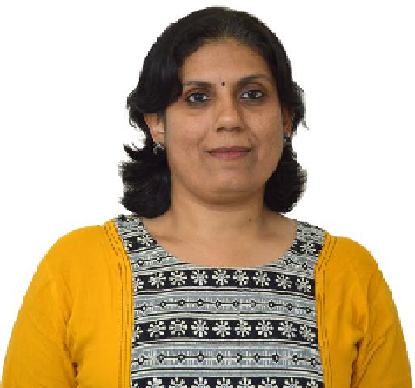
\includegraphics{src/Figures/authors/Aparna-Gooru-Lab.png}} & 

\centerline{\large\bf Aparna Lalingkar}

\bigskip
Before joining Gooru Labs. Before joining Gooru labs, She was a postdoctorate research fellow at University of Haifa, Israel under the fellowship of Planning and Budgeting Commission of Israeli Higher Education.

\bigskip

She is a mathematician and educational technologist with PhD in Information Technology. For PhD she had proposed an ontology for teaching problem solving in mathematics. Her research interest include: application of Information Technology to Education specifically mathematics and science education, application of semantic web technology to education, ontological engineering and management, online assessment, automation of applications, educational technology and management.

\bigskip

She earned an MPhil in math education research from Cambridge University, UK and have received several academic fellowships and awards including HP Labs fellowship for PhD, DFID \& CCT fellowship for MPhil.

\bigskip

She has wide range of teaching and work experience. She has taught to tribal students as well as intellectually gifted students. She has also taught graduate level and master’s level students. During PhD at IIITB, she has mentored MTech students for some projects.\\

\raisebox{-4.4cm}{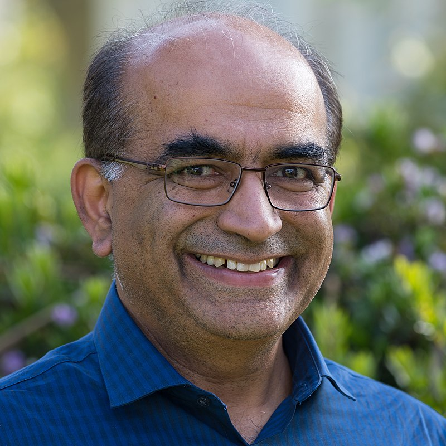
\includegraphics{src/Figures/authors/Prasad_Ram,_June_2019.png}} & 

\centerline{\large\bf Prasad Ram}

\bigskip
Prasad Ram (aka Pram) is the Founder, CEO and Chairman of Gooru. While working at Google, Pram devised a prototype to address his problem of finding age and topic appropriate educational resources on the web. Gooru, as it is today, began as a “20\% effort” evolved into a year-long pilot in India that included 1,000 students across 25 classrooms. Pram left Google to pursue Gooru as a non-profit education technology start-up. Pram has previously worked at Xerox Research, Dynamx Technology (co-founder), Yahoo! and Google. Pram has a Ph.D. and M.S. in Computer Science from UCLA, and he obtained his B.Tech. in Computer Science from IIT-Bombay. You can reach Pram at pram@gooru.org.\\
&\\  
\clineB{1-2}{2.5}
\end{tabular}


\newpage

\noindent
\begin{tabular}{V{2.5}cp{13.8cm}V{2.5}}
\clineB{1-2}{2.5}
 &\\

\raisebox{-4.2cm}{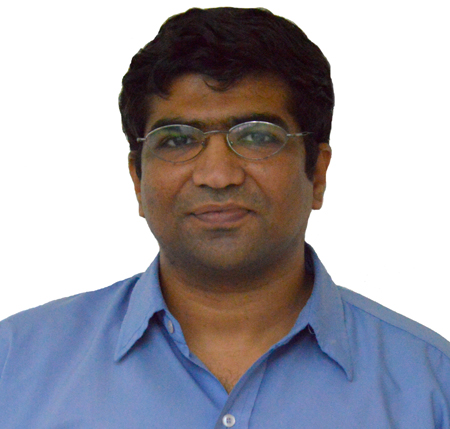
\includegraphics{src/Figures/authors/srinath_srinivasa.png}} & 

\centerline{\large\bf Prof. Srinath Srinivasa}

\bigskip
Heads the Web Science lab and is the Dean (R\&D) at IIIT Bangalore, India. Srinath holds a Ph.D. (magna cum laude) from the Berlin Brandenburg Graduate School for Distributed Information Systems (GkVI) Germany. He holds an M.S. (by Research) degree from IIT-Madras and a B.E. degree in Computer Science and Engineering from The National Institute of Engineering (NIE) Mysore. He works in the area of Web Science — that models of the impact of the web on humanity. Technology for educational outreach and social empowerment has been a primary motivation driving his research. He has participated in several initiatives for technology-enhanced education including the VTU Edusat program, The National Programme for Technology Enhanced Learning (NPTEL) and an educational outreach program in collaboration with Upgrade.

\bigskip

He is a member of various technical and organizational committees for international conferences like International Conference on Weblogs and Social Media (ICWSM), ACM Hypertext, COMAD/CoDS, ODBASE, etc. He is also a life member of the Computer Society of India (CSI). As part of academic community outreach, Srinath has served on the Board of Studies of Goa University and as a member of the Academic Council of the National Institute of Engineering, Mysore. He has served as a technical reviewer for various journals like the VLDB journal, IEEE Transactions on Knowledge and Data Engineering, and IEEE Transactions on Cloud Computing. He is also the recipient of various national and international grants for his research activities.\\

&\\
\clineB{1-2}{2.5}
\end{tabular}

\vskip 1cm

\begin{figure}[H]
\centering

\includegraphics[scale=.15]{src/Figures/QR-codes/qr-code_characterization-of.png}

\medskip

{\large\sf Access this article on the Web}
\end{figure}
